\chapter{Objects and selections}
\label{chap:objects}

\section{Jets, MET}

\subsection{Jets}
Jets are reconstructed from charged PF candidates clustered with the
anti-$\mathrm{k_t}$ algorithm~\cite{CMS:Cacciari2008gp, CMS:Cacciari2011ma}
using a distance parameter of 0.4. Charged particles
not originating from the primary vertex (PV), taken to be the reconstructed vertex with the largest value of $\Sigma \pt^2$,
are removed before clustering the jets. While this is a direct mitigation of the effect of 
pileup, the jet \pt, calculated as the vector sum
of the constituent PF candidates, is susceptible to further contributions from pileup
and detector effects. However, jet energy corrections, primarily
parameterized by jet \pt and $\eta$, are derived using data and simulation to
counteract these effects on a jet-by-jet basis~\cite{CMS:Khachatryan2016kdb, CMS:PASJME16003}.

Additional jet selections (tight jet identification) are applied to reject
pathological jets. For data collected during 2016, they are
\begin{itemize}
    \item neutral hadronic energy fraction $<$ 0.99
    \item neutral electromagnetic energy fraction $<$ 0.99
    \item number of constituents $>$ 1
    \item charged hadronic energy fraction $>$ 0
    \item charged multiplicity $>$ 0
    \item charged electromagnetic energy fraction $>$ 0
\end{itemize}
\noindent and for data collected during 2017 and 2018, the selections are
\begin{itemize}
    \item neutral hadronic energy fraction $<$ 0.9
    \item neutral electromagnetic energy fraction $<$ 0.9
    \item number of constituents $>$ 1
    \item charged hadronic energy fraction $>$ 0
    \item charged multiplicity $>$ 0
\end{itemize}


To avoid double counting of objects,
selected jets are those that do not overlap with analysis leptons 
(within a cone of $\Delta R \equiv \sqrt{\Delta\eta^2 + \Delta\phi^2} = 0.4$),
and have $\pt>40\GeV$ and $|\eta|<2.4$. The multiplicity of selected jets
is defined to be \Njets. The scalar sum of selected jet \pt
is called \HT.

\subsection{B-tagging}
Many of the SUSY models probed in this analysis have a high multiplicity of
top quarks; SM four top quark production has four. Each top quark decays into
a b quark and W boson, so jets arising from b quarks are an important object
to efficiently identify. Hadrons containing b quarks have lifetimes that
allow them to travel on the order of a millimeter from the collision before
decaying, creating tracks pointing to a secondary vertex. We use a deep
neural network algorithm, DeepCSV~\cite{CMS:Sirunyan2017ezt}, which makes use
of information such as tracks and secondary vertices to produce a
discriminating value for b jets. A threshold value (the medium working point)
on this discriminant is set such that the efficiency to correctly identify a
b jet is approximately 65\% for jet \pt around 40\GeV while maintaining a
misidentification rate of 1\% for light-flavor jets (udsg).
While they are not directly used here, there are two additional working points
for the b-tagging, loose and tight, which have 10\% and 0.1\% misidentification 
rates for light-flavor jets, respectively.

This \Nbjets variable is defined as the multiplicity 
of b-tagged jets with $\pt>25\GeV$ and $|\eta|<2.4$ which are
not overlapping with leptons. The lower threshold compared
to nominal jets above allows for increased signal acceptance for softer event
topologies.

On top of the jet-by-jet corrections, event-level weights, known as 
b tag scale factors, are applied to bring data and simulation \Nbjets into agreement,
and they are derived by effectively reshaping the DeepCSV discriminator
distribution~\cite{CMS:BtagSF}.

\subsection{MET}

The missing transverse energy,
equivalently referred to as MET, $\slashed{E}_\mathrm{T}$, or $\ptmiss$, is defined
as the magnitude of the negative of the vectorial sum of the $\vec{p_\mathrm{T}}$ of PF candidates in an
event~\cite{CMS:Sirunyan2019kia}.

The MET has a Type-I correction applied, which fully propagates
the jet energy corrections into the computation:

\begin{equation}
    \vec{\slashed{E}}_\mathrm{T}
    = \vec{\slashed{E}}_\mathrm{T}^\mathrm{raw}
    - \sum_{\mathrm{jets}} \left( 
        \vec{p}_\mathrm{T,jet}^\text{corr} 
        - \vec{p}_\mathrm{T,jet}
    \right)
\end{equation}

Additional event-level filters detailed in \cite{CMS:JetMETFilters} are applied 
to reject pathological events associated with misreconstruction, or sources of 
detector noise.

\section{Leptons}

\subsection{Identification}

Muons are reconstructed by combining information from tracker hits
with those in the muon system to form a global fit.
The base identification criteria for reconstructed muons is encapsulated in the 
``medium muon ID''~\cite{CMS:Sirunyan2019yvv} and requires
a certain level of quality in the tracker and muon system track matching.

Analysis muons must have $\pt>10\GeV$ and $|\eta|<2.4$. 
We require that muons have a relative 
uncertainty less than 20\% on the reconstructed momentum ($\delta \pt/\pt<0.2$).
This helps ensure that the charge of the muon track has not been misreconstructed.

Analysis electrons must have $\pt>15\GeV$ and $|\eta|<2.5$.
Electrons are identified by constructing a boosted decision tree (BDT) with
a variety of variables tied to the track
and ECAL deposits used to reconstruct the electron~\cite{CMS:Khachatryan2015hwa}.
These include 
\begin{itemize}
    \item ECAL shower-shape variables
    \begin{itemize}
    \item $\sigma_{i\eta i\eta}$ (weighted width of shower along $\eta$)
    \item $\sigma_{i\phi i\phi}$ (weighted width of shower along $\phi$)
    \item cluster circularity
    \item cluster $\eta$, $\phi$ widths
    \item $\mathrm{R_9}$, the ratio of energy in 3x3 to 5x5 set of towers surrounding the seed crystal
    \item H/E, the ratio of (adjacent) HCAL energy to ECAL deposits
    \end{itemize}
    \item track-cluster matching variables
    \begin{itemize}
    \item $E/p_\mathrm{in}$, $E/p_\mathrm{out}$, where $p_\mathrm{in/out}$ is the innermost/outermost track momentum
    \item $\Delta \eta_\mathrm{in}$ ($\eta$ difference between cluster and inner track)
    \item $\Delta \eta_\mathrm{out}$
    \item $\Delta \phi_\mathrm{in}$ ($\phi$ difference between cluster and inner track)
    \item $|1/E_\mathrm{clust} - 1/p|$
    \end{itemize}
    \item track variables
    \begin{itemize}
    \item $\chi^2$ quality of combinatorial track finder (CTF) and Gaussian-sum filter (GSF) tracks
    \item number of CTF and GSF hits
    \item $(p_\mathrm{in}-p_\mathrm{out})/p_\mathrm{in}$, fraction of energy lost through Brehmsstrahlung
    \end{itemize}
\end{itemize}

The BDT discriminant is converted into a boolean decision per lepton with
working points depending on the year and $\pt$, which will not be shown here 
for the sake of brevity. We simply take and refer to two boolean decisions
as the ``loose'' and ``tight" working points, where the tight WP has
relatively lower efficiency to select electrons,
but also a lower efficiency to misidentify
other objects as electrons.

For electrons, we additionally consider a conversion veto that locates and rejects $\gamma \rightarrow e^{+} e^{-}$,
and a ``number of expected missing inner hits'' variable, which is the number of 
detector hits in the inner tracker which should have registered a hit but did not.
Electrons must have no such missing hits.
Electrons must also have agreement between three different methods used to compute the charge~\cite{CMS:AN14164}.

For both electrons and muons, we require $|d_\mathrm{xy}| < 0.05\unit{cm}$,
$|d_\mathrm{z}| < 0.1\unit{cm}$,
$\mathrm{SIP}_\mathrm{3D} < 4$. The variables $|d_\mathrm{xy}|$ and $|d_\mathrm{z}|$ are the transverse and longitudinal
displacements between the PV and the point of closest approach (PCA) of the lepton's 
track, respectively. The 3D impact parameter significance, $\mathrm{SIP}_\mathrm{3D}$,
is defined as the 3D displacement between the PCA and PV divided by the measurement uncertainty.
These variables and selections make sure the leptons are produced in a prompt fashion.

The final lepton reconstruction and identification efficiency is between
45\% and 70\% for electrons with $\pt > 25\GeV$, and between 70\% and 90\%
for muons in the same momentum range. In the lower momentum range of 15-25\GeV
for electrons, the efficiency is 40\%, and in the range of 10-25\GeV for muons,
the efficiency is 55\%. 

\subsection{Isolation}

Conceptually, a lepton can be labeled isolated if the ratio of 
energy in a cone surrounding the lepton to the energy of the lepton itself
(``relative isolation'') is below a certain threshold.
However, we instead use three more sophisticated variables, improving upon this concept for robustness,
to classify leptons as isolated:
\begin{itemize}
    \item ``mini-isolation'' $\miniiso$: 
    \begin{equation}
        \miniiso = \frac{\sum_R \pt(h^\pm) - \mbox{max}(0, \sum_R \pt(h^0)+\pt(\gamma) - \rho\mathcal{A}\left(R/0.3\right)^2}{\pt(\ell)}.
    \end{equation}
    where $\rho$ is the event-level energy density from pileup,
    and $\sum_R\pt(h^\pm)$, $\sum_R\pt(h^0)$, $\sum_R\pt(\gamma)$ 
    are the sums of the $\pt$ of charged hadrons, neutral hadrons, and photons, respectively.
    The sum is performed within a lepton \pt-dependent cone of radius $R$, decreasing in size
    for higher lepton \pt:
    \begin{equation}
        R = \frac{10}{\mbox{min}(\mbox{max}(\pt(\ell), 50), 200)}
    \end{equation}
    The effective areas $\mathcal{A}$ are constants calculated in coarse bins of
    lepton $\eta$ such that the last term of the numerator represents the
    contribution from pileup and is subtracted off.
    Requiring $\miniiso$ to be below a particular value ensures that the
    lepton is isolated.

    \item \ptratio, defined as the ratio of the lepton \pt to the
    \pt of the jet geometrically closest to, or containing, the lepton:
    \begin{equation}
        \ptratio = \frac{\pt(\ell)}{\pt(\text{jet})}
    \end{equation}
    In order to avoid an
    over-correction on prompt leptons, the application of the jet energy
    correction to mitigate is only applied on the hadronic part of the jet.
    That is, the denominator of $\ptratio$ is corrected for pileup effects
    after the lepton is subtracted out, and the lepton is subsequently added back.

    \item \ptrel:
    \begin{equation}
        \ptrel=\frac{\left|\left(\vec{p}(\text{jet})-\vec{p}(\ell)\right) 
        \times \vec{p}(\ell)\right| }{|\vec{p}(\text{jet})-\vec{p}(\ell)|}
    \end{equation}
    This variable is a measure of the relative transverse separation between the lepton 
    and matching jet. For leptons arising from the decay of B mesons, for example,
    this quantity exhibits a kinematic cutoff of a few GeV. For leptons that
    happen to overlap accidentally with jets, \ptrel compares two uncorrelated
    quantities and exhibits no kinematic cutoff, so this quantity can be large.
    This property allows us to recover leptons that would be labeled non-isolated
    by the previous two variables.
\end{itemize}

Using the above three variables, we classify a lepton
as isolated if the following boolean condition is satisfied:
\begin{equation}
  \miniiso < I_1 \wedge ( \ptratio > I_2 \vee \ptrel > I_3 )
\end{equation}
where $I_i$ threshold values depend on the lepton flavor and PU conditions
of the flavor of the lepton. These values are tabulated in Table~\ref{tab:isoWPs}.

\begin{table}[h]
    \label{tab:isoWPs}
    \centering
    {\renewcommand{\arraystretch}{1.3}
    \begin{tabular}{l|cccc}
        \hline
        & e/$\mu$ loose WP &  $\mu$ tight WP & e tight WP \\ \hline 
        $I_1$ & 0.4 & 0.16 (2016), 0.11 (2017/2018) & 0.12 (2016), 0.07 (2017/2018) \\
        $I_2$ & 0  & 0.76 (2016), 0.74 (2017/2018) & 0.80 (2016), 0.78 (2017/2018) \\
        $I_3$ (\GeVns) & 0  & 7.2 (2016), 6.8 (2017/2018) & 7.2 (2016), 8.0 (2017/2018) \\ \hline
    \end{tabular}}
    \caption{Isolation working points }
\end{table}

\section{Other variables}

We make use of the minimum transverse mass ($\mtmin$) which is defined as:
\begin{equation}
    \mtmin = \mathrm{min}\left[ \mT(\ell_1, \ETm), \mT(\ell_2, \ETm)\right ]
\end{equation}
where a single transverse mass term is given by
\begin{equation}
    \mtmin = \sqrt{2\pt(\ell) \ETm (1-\cos\Delta \phi_{\ell,\ETm})}
\end{equation}
and $\Delta \phi_{\ell,\ETm}$ is the azimuthal separation between the lepton
and the \ptmiss vector.

For events where \ptmiss arises primarily from neutrinos from W boson decays,
as is the case with the pervasive $\ttbar$ and $W$ processes, this variable
has a kinematic cutoff at the W boson mass, $m_{W}$. Signal events
where the \ptmiss is generated from an energetic $\lsp$ particle
will not exhibit such a kinematic cutoff.

Figure~\ref{fig:mtminttbar} shows the distribution of $\mtmin$ for a signal hypothesis \Totttt and the
\ttbar background, with the W boson mass marked as a vertical line. It is clear that 
the \ttbar background is almost completely bounded by the W mass, while the signal has a
large tail extending beyond the W mass.

\begin{figure}[!hbtp]
\centering
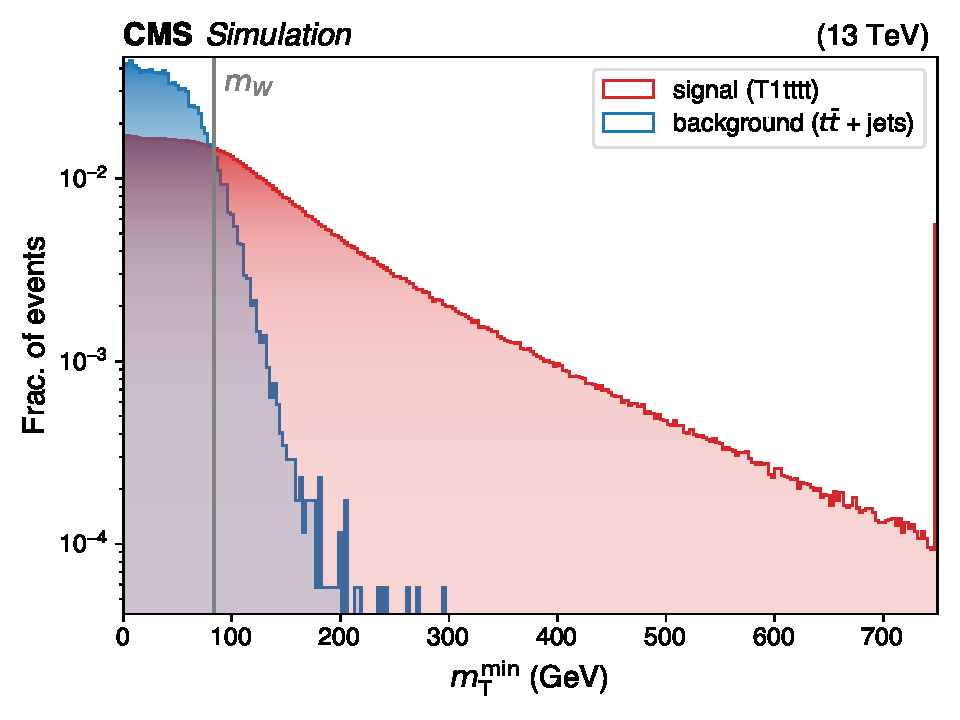
\includegraphics[width=.75\textwidth]{figs/misc/mtmin_signal_ttbar}
\caption{
    Normalized distribution of $\mtmin$ shown for signal hypothesis \Totttt and 
    \ttbar background.
}
\label{fig:mtminttbar}
\end{figure}

\section{Trigger}

Clearly before one can analyze events, one must have collected them with the detector first.
Triggers are meant to identify and save interesting events in data while making sure to not to overwhelm
the readout hardware, reconstruction software, and storage used by CMS. 
Same-sign searches make use of dilepton triggers
which require at least two leptons at trigger level of a given $\pt$, usually along with some
isolation quantities or $\HT$. For a given trigger rate, 
the more stringent the requirements on isolation or $\HT$, the
lower the thresholds on lepton $\pt$.

In the SUSY analysis, based on trigger thresholds, 
we only consider muons (electrons) with \pt of at least 10 (15) \GeV.
For events with lepton $\pt < 25\GeV$ for both SS leptons, the set of signal triggers, depending on year
and SS lepton pair flavor, is given in Table~\ref{tab:sstrigslow}, otherwise, the signal triggers in 
Table~\ref{tab:sstrigshigh} are used.
For example, the HLT\_Ele23\_Ele12\_CaloIdL\_TrackIdL\_IsoVL\_DZ trigger
requires at least one electron with $\pt>23~\GeV$ and another with $\pt>12~\GeV$,
which meet some loose amount of identification and isolation criteria and a
cut on $d_\mathrm{z}$. For other triggers, the substring ``PFHT350'' specifies a requirement
of $\HT>350~\GeV$ at the HLT. Note that there is no pair charge enforced by the trigger, 
so both opposite- and same-sign pairs can pass these dilepton triggers.

The \smft analysis considers muons and electrons with \pt of at least 20 \GeV. As a result,
the modified signal trigger strategy summarized in Table~\ref{tab:fttrigs} is used.

A set of single lepton triggers, listed in Table~\ref{tab:frtrigs},
is used for the estimation of the fake rate, which
will be discussed in the following chapter.

\begin{table}[h!]
\label{tab:sstrigslow}
 \begin{center}  
\caption{Summary of the signal triggers for the SUSY analysis with low lepton $\pt$}
\resizebox{0.99\textwidth}{!}{
 \begin{tabular}{|c|c|}\hline 
 \multicolumn{2}{|c|}{2016} \\\hline
Final state        & Trigger Name                                                   \\ \hline
Same sign $\mu\mu$ & HLT\_DoubleMu8\_Mass8\_PFHT300                         \\
Same sign $ee$     & HLT\_DoubleEle8\_CaloIdM\_TrackIdM\_Mass8\_PFHT300     \\
Same sign $e\mu$   & HLT\_Mu8\_Ele8\_CaloIdM\_TrackIdM\_Mass8\_PFHT300      \\
\hline\hline
 \multicolumn{2}{|c|}{2017} \\\hline
Final state        & Trigger Name                                                   \\ \hline
Same sign $\mu\mu$ & HLT\_DoubleMu4\_Mass8\_DZ\_PFHT350                     \\
Same sign $ee$     & HLT\_DoubleEle8\_CaloIdM\_TrackIdM\_DZ\_Mass8\_PFHT350 \\
Same sign $e\mu$   & HLT\_Mu8\_Ele8\_CaloIdM\_TrackIdM\_Mass8\_PFHT350\_DZ  \\
\hline\hline
 \multicolumn{2}{|c|}{2018} \\\hline
Final state        & Trigger Name                                                   \\ \hline
Same sign $\mu\mu$ & HLT\_DoubleMu4\_Mass8/3p8\_DZ\_PFHT350                 \\
Same sign $ee$     & HLT\_DoubleEle8\_CaloIdM\_TrackIdM\_DZ\_Mass8\_PFHT350 \\
Same sign $e\mu$   & HLT\_Mu8\_Ele8\_CaloIdM\_TrackIdM\_Mass8\_PFHT350\_DZ  \\
\hline
\end{tabular}
 }
\end{center}
\end{table}


\begin{table}[h!]
\label{tab:sstrigshigh}
\begin{center}  
\caption{Summary of the signal triggers for the SUSY analysis with high lepton $\pt$}
\resizebox{0.99\textwidth}{!}{
 \begin{tabular}{|c|c|}\hline 
 \multicolumn{2}{|c|}{2016} \\\hline
Final state        & Trigger Name                                                          \\ \hline
Same sign $\mu\mu$ & HLT\_(Tk)Mu17\_TrkIsoVVL\_(Tk)Mu8\_TrkIsoVVL(\_DZ)            \\
Same sign $ee$     & HLT\_Ele23\_Ele12\_CaloIdL\_TrackIdL\_IsoVL\_DZ               \\ 
Same sign $e\mu$   & HLT\_Mu23/8\_TrkIsoVVL\_Ele12/23\_CaloIdL\_TrackIdL\_IsoVL\_DZ\\
\hline\hline
 \multicolumn{2}{|c|}{2017} \\\hline
Final state        & Trigger Name                                                          \\ \hline
Same sign $\mu\mu$ & HLT\_Mu17\_TrkIsoVVL\_Mu8\_TrkIsoVVL\_DZ(\_Mass3p8)           \\
Same sign $ee$     & HLT\_Ele23\_Ele12\_CaloIdL\_TrackIdL\_IsoVL                   \\ 
Same sign $e\mu$   & HLT\_Mu23/8\_TrkIsoVVL\_Ele12/23\_CaloIdL\_TrackIdL\_IsoVL\_DZ\\
\hline\hline
 \multicolumn{2}{|c|}{2018} \\\hline
Final state        & Trigger Name                                                          \\ \hline
Same sign $\mu\mu$ & HLT\_Mu17\_TrkIsoVVL\_Mu8\_TrkIsoVVL\_DZ\_Mass3p8             \\
Same sign $ee$     & HLT\_Ele23\_Ele12\_CaloIdL\_TrackIdL\_IsoVL                   \\ 
Same sign $e\mu$   & HLT\_Mu23/8\_TrkIsoVVL\_Ele12/23\_CaloIdL\_TrackIdL\_IsoVL\_DZ\\
\hline
\end{tabular}
 }
\end{center}
\end{table}


\begin{table}[h!]
\label{tab:fttrigs}
 \begin{center}  
\caption{Summary of the signal triggers for the \smft analysis}
\resizebox{0.99\textwidth}{!}{
 \begin{tabular}{|c|c|}\hline 
 \multicolumn{2}{|c|}{2016} \\\hline
Final state        & Trigger Name                                                   \\ \hline
Same sign $\mu\mu$ & HLT\_DoubleMu8\_Mass8\_PFHT300                         \\
Same sign $ee$     & HLT\_DoubleEle8\_CaloIdM\_TrackIdM\_Mass8\_PFHT300     \\
Same sign $e\mu$   & HLT\_Mu8\_Ele8\_CaloIdM\_TrackIdM\_Mass8\_PFHT300      \\
\hline\hline
 \multicolumn{2}{|c|}{2017} \\\hline
Final state        & Trigger Name                                                   \\ \hline
Same sign $\mu\mu$ & HLT\_Mu17\_TrkIsoVVL\_Mu8\_TrkIsoVVL\_DZ(\_Mass8)             \\
Same sign $ee$     & HLT\_Ele23\_Ele12\_CaloIdL\_TrackIdL\_IsoVL                   \\ 
Same sign $e\mu$   & HLT\_Mu23/8\_TrkIsoVVL\_Ele12/23\_CaloIdL\_TrackIdL\_IsoVL\_DZ\\
\hline\hline
 \multicolumn{2}{|c|}{2018} \\\hline
Final state        & Trigger Name                                                   \\ \hline
Same sign $\mu\mu$ & HLT\_Mu17\_TrkIsoVVL\_Mu8\_TrkIsoVVL\_DZ\_Mass3p8             \\
Same sign $ee$     & HLT\_Ele23\_Ele12\_CaloIdL\_TrackIdL\_IsoVL                   \\ 
Same sign $e\mu$   & HLT\_Mu23/8\_TrkIsoVVL\_Ele12/23\_CaloIdL\_TrackIdL\_IsoVL\_DZ\\
\hline
\end{tabular}
 }
\end{center}
\end{table}



\begin{table}[h!]
\label{tab:frtrigs}
\caption{Summary of the control triggers used for the fake rate measurement}
\begin{center}
% \resizebox*{1\textwidth}{!}{
\begin{tabular}{|c|c|}\hline
Final state                                    & Trigger Name \\\hline
$\mu$ (isolated trigger leg)     & HLT\_Mu8/17\_TrkIsoVVL\\
$\mu$ (non isolated trigger leg) & HLT\_Mu8/17\\
$e$ (isolated trigger leg)       & HLT\_Ele12/23\_CaloIdL\_TrackIdL\_IsoVL\_PFJet30\\
$e$ (non isolated trigger leg)   & HLT\_Ele8/17\_CaloIdM\_TrackIdM\_PFJet30\\
\hline
\end{tabular}
% }
\end{center}
\end{table}


\FloatBarrier

Triggers are required for all events in data and simulation, and residual
differences are corrected via trigger scale factors, which are applied to
simulation to bring agreement with data. These scale factors are computed via
the tag and probe method~\cite{CMS:TagAndProbe}
to measure the efficiencies in data and simulation
before taking the ratio. Efficiencies for dilepton triggers are the product
of efficiencies for individual lepton selections (``lepton legs''). The tag
and probe method defines the efficiency for a lepton leg as the number of
events where the probed lepton candidate matches the studied lepton leg
within $\Delta R$ of 0.4, divided by the total number of selected events. 

For example, to measure the efficiency for the isolated Mu17 leg of the 
dimuon trigger in 2018 data from Table~\ref{tab:sstrigshigh}, we 
first select events firing the HLT\_IsoMu27 trigger in the 
single muon dataset. Tag and probe pairs within the Z boson mass window
are required to pass the offline analysis lepton selection to reduce 
the fake contribution and eliminate the need for parametric fits.
The efficiency for the trigger leg is then calculated as the probability 
for the probe to pass the Mu17 leg selections. These efficiencies in data and 
simulation are shown as a function of
muon \pt in Fig.~\ref{fig:triggermuonpt}. Their ratio, in the bottom panel,
is the trigger efficiency for this lepton leg and is within 1\% of unity
in the plateau region of muon $\pt > 20\GeV$.
The actual scale factors are derived in bins of \pt and $\eta$, 
for each of the three years, and each of the triggers.

\begin{figure}[!hbtp]
\centering
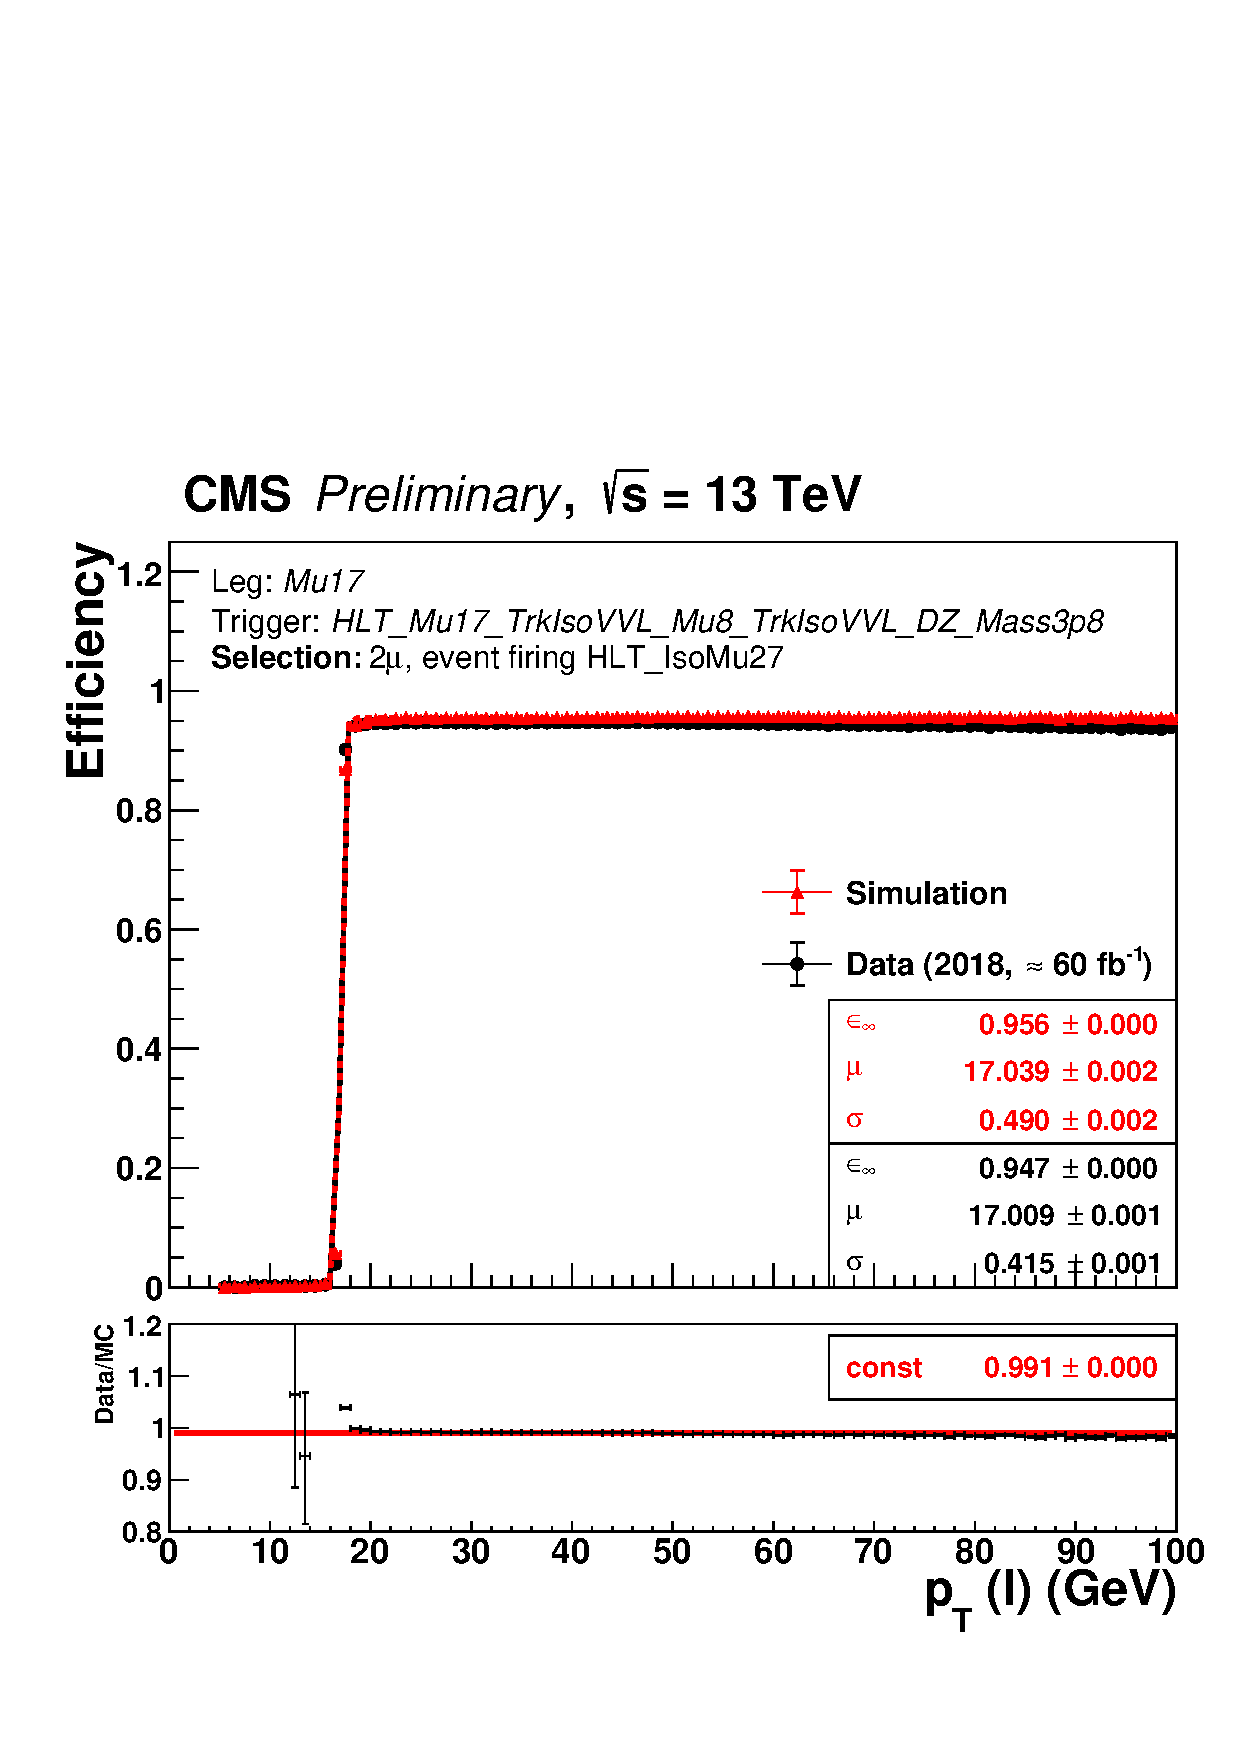
\includegraphics[width=.70\textwidth]{figs/ssan/eff_1d_mu17_2018}
\caption{
    Efficiencies for the leading Mu17 leg of the high \pt isolated 
    dimuon trigger used in 2018, separately for data and simulation.
}
\label{fig:triggermuonpt}
\end{figure}

\FloatBarrier

\section{Baseline selections}

With the objects in place, we can now discuss the baseline selections used for the 
inclusive SUSY analysis and the more restricted \smft analysis.
As the title of this thesis suggests, both require the presence of at least
two leptons (electrons or muons) with the same charge. 
Appropriate triggers are required for data and all simulation.
Subsequent
requirements on $\HT$, $\Njets$, $\Nbjets$, $\ptmiss$, and the leading/trailing lepton \pt are listed in 
Table~\ref{tab:baselineselections}.

\begin{table}[h]
    \label{tab:baselineselections}
    \centering
    \caption{Summary of baseline selections}
    {\renewcommand{\arraystretch}{1.2}
    \begin{tabular}{|l|c|c|}
        \hline
        variable &  SUSY analysis & \smft analysis \\ \hline 
        \Njets & $\geq 2$  & $\geq 2$  \\
        \Nbjets & $\geq 0$  & $\geq 2$  \\
        \HT & $\geq 80~\GeV$  & $\geq 300~\GeV$  \\
        \ptmiss & $>0~\GeV$  & $>50~\GeV$  \\
        $\pt(\ell_1)$ & $>15/10~\GeV$ (e/$\mu$)  & $>25~\GeV$  \\
        $\pt(\ell_2)$ & $>15/10~\GeV$ (e/$\mu$)  & $>20~\GeV$  \\
        \hline
    \end{tabular}}
\end{table}

To reduce the background from production of low-mass resonances with
charge-misidentified electrons, events that have a same-sign electron pair with invariant mass lower than 12\GeV
are rejected. 

For the SUSY analysis, we reject events with same-flavor lepton pairs
that have an invariant mass ($m_{\ell\ell}$) less than 12\GeV. Such a selection
reduces backgrounds arising from decays of b-hadrons, c-hadrons, and the Drell-Yan (DY)
process ($\PZ/\gamma^\star\rightarrow \ell^\pm \ell^\mp$).

For the \smft analysis, events where a third lepton is identified with $\pt>7\GeV$ for electrons
or $\pt>5\GeV$ for muons and which forms an opposite-sign (OS) same-flavor pair
with $m_{\ell\ell}<12\GeV$ or in the range of 76-106\GeV are also rejected.
However, for events with invariant mass in the range of 76-106\GeV where
the $\pt>20\GeV$ for the third lepton, 
this resonance veto is inverted
and these events are instead used for a background control region 
enriched in $\ttZ$ (CRZ) to be discussed in more detail in the next
section. If a Z candidate is not found, a third tight lepton present in an event
with $\pt>20\GeV$ contributes to the lepton multiplicity, $\Nleps$, which 
starts at a value of 2 by virtue of the same-sign selection.

\section{Event-level BDT}

For the more targeted SM four top quark analysis, a BDT is used to increase the signal to
background ratio.

The BDT classifier utilizes a gradient boosting algorithm 
implemented using the xgboost framework~\cite{MISC:xgboost}
to train 500 trees
with a depth of 4 using simulation, and is based on the following 19
variables:
\begin{enumerate}
    \item \Njets
    \item \Nbjets (nominal, medium WP)
    \item \Nleps
    \item \ptmiss
    \item \Nbjets (calculated with the loose WP)
    \item \Nbjets (calculated with the tight WP)
    \item scalar \pt sum of b-tagged jets
    \item $p_\mathrm{T}(\ell_1)$
    \item $p_\mathrm{T}(\ell_2)$
    \item $p_\mathrm{T}(\ell_3)$
    \item $p_\mathrm{T}(\mathrm{j}_1)$  (leading jet)
    \item $p_\mathrm{T}(\mathrm{j}_6)$ (jet with sixth highest \pt)
    \item $p_\mathrm{T}(\mathrm{j}_7)$ (jet with seventh highest \pt)
    \item $p_\mathrm{T}(\mathrm{j}_8)$ (jet with eighth highest \pt)
    \item $\Delta\phi(\ell_1,\ell_2)$
    \item $\Delta\eta(\ell_1,\ell_2)$
    \item $m(\ell_1,\mathrm{j}_1)$
    \item $q(\ell_1)$ (charge of the leading lepton)
    \item $\mathrm{max}(m(j_\mathrm{i})/\pt(j_\mathrm{i}))$ over all selected jets in an event
\end{enumerate}

The charge of the leading lepton provides a discrimination handle against SM processes which are
charge asymmetric due to the LHC preferring positive charge initial states.
The maximum ratio of jet mass to \pt allows a handle to find jets which clustered together 
multiple decay products of a top quark, for example.

The variables were iteratively chosen from a larger pool of kinematic variables by selecting
the most performant variables and retraining until the performance started to suffer.

Training was performed on simulation with a loosened \smft baseline selection 
to prevent issues with training by increasing statistics:
\begin{itemize}
    \item $\Nbjets \geq 2$
    \item $\HT \geq 300~\GeV$
    \item $\ptmiss>50~\GeV$
    \item $\pt(\ell_1)>15~\GeV$
    \item $\pt(\ell_2)>15~\GeV$
\end{itemize}

The raw discriminant values for signal and background separated into test and train sets
is shown in Fig.~\ref{fig:xgboostdisc}. There is little to no overtraining
observed.

\begin{figure}[!hbtp]
\centering
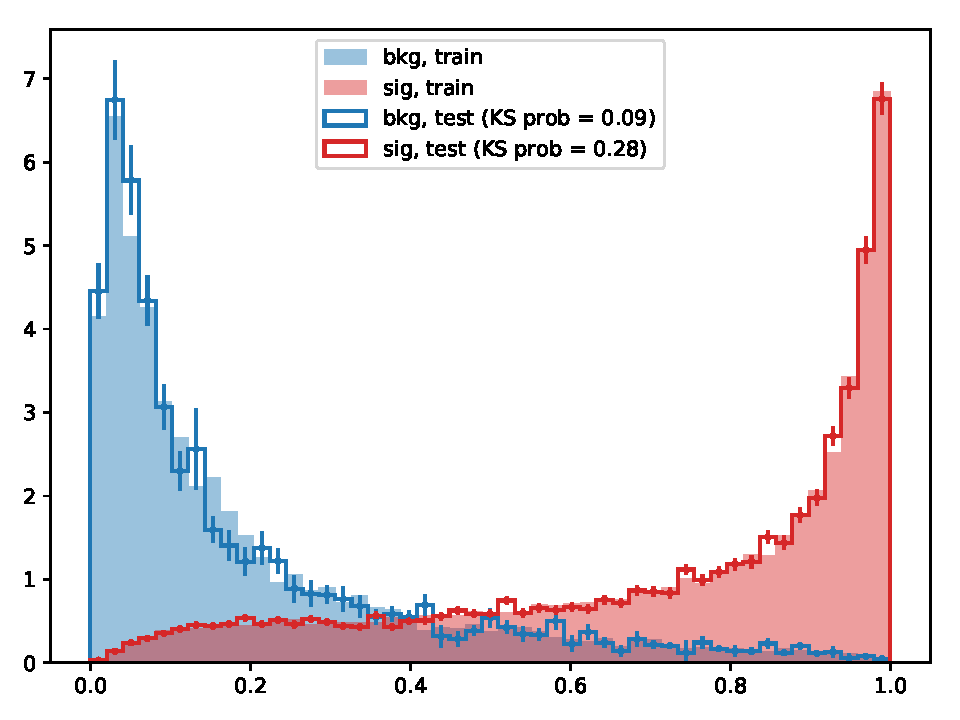
\includegraphics[width=.70\textwidth]{figs/ftan/xgboostdisc}
\caption{
    Raw discriminant values for training and testing sets.
}
\label{fig:xgboostdisc}
\end{figure}

\FloatBarrier

\section{Signal regions}

\subsection{SUSY analysis}

Following the SUSY analysis baseline selection, we define 
six exclusive categories depending on the kinematics of event and the leptons:
\begin{itemize}
\item High-High SS pair (HH): exactly 2 leptons, both with $\pt>25 \GeV$, and $\ptmiss>50 \GeV$;
\item High-Low SS pair (HL): exactly 2 leptons, one with $\pt>25 \GeV$, one with $\pt<25 \GeV$, and $\ptmiss>50 \GeV$;
\item Low-Low SS pair (LL): exactly 2 leptons, both with $\pt<25 \GeV$ and $\ptmiss>50 \GeV$;
\item Low \ptmiss (LM): exactly 2 leptons, both with $\pt>25 \GeV$, and $\ptmiss<50 \GeV$; and
\item Multilepton with an on-shell Z boson (on-\PZ ML): $\geq$3 leptons, at least one with $\pt>25 \GeV$, $\ptmiss>50 \GeV$, $\geq 1$ \PZ boson candidate formed by a pair of OS, same-flavor leptons with $76 < m_{\ell\ell}< 106 \GeV$.
\item Multilepton without an on-shell Z boson (off-\PZ ML): same as on-\PZ ML but without a \PZ boson candidate.
\end{itemize}

For the on-\PZ ML category, the calculation of $\mtmin$ uses leptons not 
forming the Z candidate.

The categories are structured to be generally sensitive to different SUSY models
considered in the analysis. For example, the HH category gives sensitivity
to many of the scenarios with large mass splittings between the 
gluino and lightest neutralino (\Totttt, \TfttbbWW, \Tftttt, \TfqqqqWW).
Lower \pt threshold categories, HL and LL, provide sensitivity to smaller 
mass splittings, resulting in less energetic leptons. Models with
Z bosons in the final state, such as \TfqqqqWZ and \TsttHZ, will typically
fall into the ML categories. The LM category captures events that
otherwise would be lost due to the $\ptmiss>50\GeV$ requirement in the
HH, HL, and LL regions, and is particularly relevant for the 
\ToqqqqL and \Totbs RPV models.


Within each category, many signal regions (SRs) are formed based on 
\Njets, \Nbjets, \HT, \ptmiss, SS charge, \mtmin.
The SRs
within the six categories, HH, HL, LL, LM, on-\PZ ML, and off-\PZ ML,
are summarized in Tables~\ref{tab:SRDefHH}, \ref{tab:SRDefHL},
\ref{tab:SRDefLL}, \ref{tab:SRDefLM}, \ref{tab:SRDefMLonZ} and
\ref{tab:SRDefMLoffZ}, respectively. 

\begin{table*}[htb!]
    \centering
            \begin{scriptsizetabular}{|c|c|c|c|c|c|c|c|c|}
                \hline
                % $\Nbjets$                             & $\MTmin$              & $\ptmiss$              & $\Njets$            & $\HT < 300$                          & $\HT\in[300, 1125]$ & $\HT\in[1125, 1300]$                  & $\HT\in[1300, 1600]$                  & $\HT > 1600$ \\ \hline \hline
                $\Nbjets$                             & $\MTmin$              & $\ptmiss$              & $\Njets$            & $\HT < 300$                          & $[300, 1125]$ & $[1125, 1300]$                  & $[1300, 1600]$                  & $ > 1600$ \\ \hline \hline
                \multirow{8}{*}{0}                & \multirow{4}{*}{$<$120}    & \multirow{2}{*}{ 50--200}  & 2--4                 & SR1                                      & SR2                     & \multirow{10}{*}{\shortstack{SR54  \\ $\Njets < 5$ }}& \multirow{10}{*}{\shortstack{SR55  \\ $\Njets < 5$ }}& \multirow{10}{*}{\shortstack{SR56  \\ $\Njets < 5$ }}\\ \cline{4-6}
                                                  &                            &                             & $\geq$5                  & \multirow{7}{*}{SR3}                     & SR4                     &                                           &                                           & \\ \cline{3-4} \cline{6-6}
                                                  &                            & \multirow{2}{*}{200--300}  & 2--4                 &                                          & SR5 (++) / SR6 (-$\,$-)   &                                           &                                           & \\ \cline{4-4} \cline{6-6}
                                                  &                            &                             & $\geq$5                  &                                          & SR7                     &                                           &                                           & \\ \cline{2-4} \cline{6-6}
                                                  & \multirow{4}{*}{$>$120}    & \multirow{2}{*}{ 50--200}  & 2--4                 &                                          & SR8 (++) / SR9 (-$\,$-)   &                                           &                                           & \\ \cline{4-4} \cline{6-6}
                                                  &                            &                             & $\geq$5                  &                                          & \multirow{3}{*}{SR10}   &                                           &                                           & \\ \cline{3-4}
                                                  &                            & \multirow{2}{*}{200--300}  & 2--4                 &                                          &                         &                                           &                                           & \\ \cline{4-4}
                                                  &                            &                             & $\geq$5                  &                                          &                         &                                           &                                           & \\ \cline{1-6}
                \multirow{8}{*}{1}                & \multirow{4}{*}{$<$120}    & \multirow{2}{*}{ 50--200}  & 2--4                 & SR11                                     & SR12                    &  \multirow{10}{*}{\shortstack{SR57 \\ $\Njets = $ 5, 6 }}& \multirow{10}{*}{\shortstack{SR58  \\ $\Njets = $ 5, 6 }}& \multirow{10}{*}{\shortstack{SR59  \\ $\Njets =  $ 5, 6}}\\ \cline{4-6}
                                                  &                            &                             & $\geq$5                  & \multirow{7}{*}{\shortstack{SR13 (++) / \\ SR14 (-$\,$-)}} & SR15 (++) / SR16 (-$\,$-) &                                           &                                           & \\ \cline{3-4} \cline{6-6}
                                                  &                            & \multirow{2}{*}{ 200--300} & 2--4                 &                                          & SR17 (++) / SR18 (-$\,$-) &                                           &                                           & \\ \cline{4-4} \cline{6-6}
                                                  &                            &                             & $\geq$5                  &                                          & SR19                    &                                           &                                           & \\ \cline{2-4} \cline{6-6}
                                                  & \multirow{4}{*}{$>$120}    & \multirow{2}{*}{ 50--200}  & 2--4                 &                                          & SR20 (++) / SR21 (-$\,$-) &                                           &                                           & \\ \cline{4-4} \cline{6-6}
                                                  &                            &                             & $\geq$5                  &                                          & \multirow{3}{*}{SR22}   &                                           &                                           & \\ \cline{3-4}
                                                  &                            & \multirow{2}{*}{ 200--300} & 2--4                 &                                          &                         &                                           &                                           & \\ \cline{4-4}
                                                  &                            &                             & $\geq$5                  &                                          &                         &                                           &                                           & \\ \cline{1-6}
                \multirow{8}{*}{2}                & \multirow{4}{*}{$<$120}    & \multirow{2}{*}{ 50--200}  & 2--4                 & SR23                                     & SR24                    &   \multirow{10}{*}{\shortstack{SR60 \\ $\Njets > 6$ }}& \multirow{10}{*}{\shortstack{SR61 \\ $\Njets > 6$ }}&\multirow{10}{*}{\shortstack{SR62 \\ $\Njets > 6$ }} \\ \cline{4-6}
                                                  &                            &                             & $\geq$5                  & \multirow{7}{*}{\shortstack{SR25 (++) / \\ SR26 (-$\,$-)}} & SR27 (++) / SR28 (-$\,$-) &                                           &                                           & \\ \cline{3-4} \cline{6-6}

                                                  &                            & \multirow{2}{*}{ 200--300} & 2--4                 &                                          & SR29 (++) / SR30 (-$\,$-) &                                           &                                           & \\ \cline{4-4} \cline{6-6}
                                                  &                            &                             & $\geq$5                  &                                          & SR31                    &                                           &                                           & \\ \cline{2-4} \cline{6-6}
                                                  & \multirow{4}{*}{$>$120}    & \multirow{2}{*}{ 50--200}  & 2--4                 &                                          & SR32 (++) / SR33 (-$\,$-) &                                           &                                           & \\ \cline{4-4} \cline{6-6}
                                                  &                            &                             & $\geq$5                  &                                          & \multirow{3}{*}{SR34}   &                                           &                                           & \\ \cline{3-4}
                                                  &                            & \multirow{2}{*}{ 200--300} & 2--4                 &                                          &                         &                                           &                                           & \\ \cline{4-4}
                                                  &                            &                             & $\geq$5                  &                                          &                         &                                           &                                           & \\ \cline{1-6}
                \multirow{6}{*}{$\geq$3}          & \multirow{4}{*}{$<$120}    & \multirow{2}{*}{ 50--200}  & 2--4 & \multirow{4}{*}{\shortstack{SR35 (++) / \\ SR36 (-$\,$-)}} & SR37 (++) / SR38 (-$\,$-) &                                           &                                           & \\ \cline{4-4} \cline{6-6}
                                                  &                            &                             & $\geq$5                    &                                          & SR39 (++) / SR40 (-$\,$-)&                                           &                                           & \\ \cline{3-4} \cline{6-6}
                                                  &                            & \multirow{2}{*}{200--300}  & 2--4 &                                          & SR37 (++) / SR38 (-$\,$-) &                                           &                                           & \\ \cline{4-4} \cline{6-6}
                                                  &                            &                             & $\geq$5                    &                                          & SR39 (++) / SR40 (-$\,$-)&                                           &                                           & \\ \cline{2-6}
                                                  & \multirow{2}{*}{$>$120}    & \multirow{2}{*}{ 50--300} & 2--4                 &\multirow{2}{*}{SR41}&SR42 (++) / SR43 (-$\,$-) &                                           &                                           & \\ \cline{4-4} \cline{6-6}
                                                  &                            &                             & $\geq$5                  &                                          & SR44 (++) / SR45 (-$\,$-)&                                           &                                           & \\ \cline{2-4} \cline{6-6}
                \hline \multirow{4}{*}{Incl.} & \multirow{4}{*}{Incl.} & 300--500                   & \multirow{2}{*}{2--4} & \multirow{4}{*}{\NA}                        & \multicolumn{4}{c|}{SR46 (++) / SR47 (-$\,$-)} \\
                \cline{3-3} \cline{6-9}           &                            & $>$500                      &                     & & \multicolumn{4}{c|}{SR48 (++) / SR49 (-$\,$-)} \\
                \cline{3-4} \cline{6-9} &  & 300--500                   & \multirow{2}{*}{$\geq$5} &                         & \multicolumn{4}{c|}{SR50 (++) / SR51 (-$\,$-)} \\
                \cline{3-3} \cline{6-9}& & $>$500                      &                     &                         & \multicolumn{4}{c|}{SR52 (++) / SR53 (-$\,$-)} \\
                \hline
        \end{scriptsizetabular}
      \caption{\label{tab:SRDefHH} The SR definitions for the HH category. Charge-split regions are indicated with (++) and (-$\,$-).
          The rightmost five columns represent a splitting in the $\HT$ variable.
        The three highest $\HT$ regions are split only by $\Njets$, resulting in 62 regions in total.
        Quantities are specified in units of \GeV where applicable.}
\end{table*}

\begin{table*}[htb!]
    \centering
            \begin{scriptsizetabular}{|c|c|c|c|c|c|c|c|}
                \hline
                $\Nbjets$                   & $\MTmin$              & $\ptmiss$              & $\Njets$             & $\HT < 300$                          & $\HT\in[300, 1125]$                                                   & $\HT\in[1125, 1300]$                  & $\HT > 1300$ \\ \hline \hline
                \multirow{4}{*}{0}          & \multirow{4}{*}{$<$120}    & \multirow{2}{*}{50--200}   & 2--4                  & SR1                                      & SR2                                                                       & \multirow{17}{*}{\shortstack{SR40 (++) / \\ SR41 (-$\,$-)}} & \multirow{17}{*}{\shortstack{SR42 (++) / \\ SR43 (-$\,$-)}} \\ \cline{4-6}
                                            &                            &                             & $\geq$5                   & \multirow{3}{*}{SR3}                     & SR4                                                                       &                                           & \\ \cline{3-4} \cline{6-6}
                                            &                            & \multirow{2}{*}{200--300}  & 2--4                  &                                          & SR5 (++) / SR6 (-$\,$-)                                                     &                                           & \\ \cline{4-4} \cline{6-6}
                                            &                            &                             & $\geq$5                   &                                          & SR7                                                                       &                                           & \\ \cline{1-6}
                \multirow{4}{*}{1}          & \multirow{4}{*}{$<$120}    & \multirow{2}{*}{ 50--200}  & 2--4                  & SR8                                      & SR9                                                                       &                                           & \\ \cline{4-6}
                                            &                            &                             & $\geq$5                   & \multirow{3}{*}{\shortstack{SR10 (++) / \\ SR11 (-$\,$-)}} & SR12 (++) / SR13 (-$\,$-)                                                   &                                           & \\ \cline{3-4} \cline{6-6}
                                            &                            & \multirow{2}{*}{ 200--300} & 2--4                  &                                          & SR14                                                                      &                                           & \\ \cline{4-4} \cline{6-6}
                                            &                            &                             & $\geq$5                   &                                          & SR15 (++) / SR16 (-$\,$-)                                                   &                                           & \\ \cline{1-6}
                \multirow{4}{*}{2}          & \multirow{4}{*}{$<$120}    & \multirow{2}{*}{ 50--200}  & 2--4                  & SR17                                     & SR18                                                                      &                                           & \\ \cline{4-6}
                                            &                            &                             & $\geq$5                   & \multirow{3}{*}{\shortstack{SR19 (++) / \\ SR20 (-$\,$-)}} & SR21 (++) / SR22 (-$\,$-)                                                   &                                           & \\ \cline{3-4} \cline{6-6}
                                            &                            & \multirow{2}{*}{ 200--300} & 2--4                  &                                          & SR23 (++) / SR24 (-$\,$-)                                                   &                                           & \\ \cline{4-4} \cline{6-6}
                                            &                            &                             & $\geq$5                   &                                          & SR25                                                                      &                                           & \\ \cline{1-6}
                \multirow{2}{*}{$\geq$3}         & \multirow{2}{*}{$<$120}    & 50--200                    & \multirow{2}{*}{$\geq$2}  & \multirow{2}{*}{\shortstack{SR26 (++) / \\ SR27 (-$\,$-)}} & SR28 (++) / SR29 (-$\,$-)                                                   &                                           & \\ \cline{3-3} \cline{6-6}
                                            &                            & 200--300                   &                      &                                          & SR30                                                                      &                                           & \\ \cline{1-6}
                Inclusive                   & $>$120                     & 50--300                    & $\geq$2                   & SR31                                     & SR32                                                                      &                                           & \\ \hline
                \multirow{4}{*}{Inclusive}  & \multirow{4}{*}{Inclusive} & 300--500                   & \multirow{2}{*}{2--4} & \multirow{4}{*}{\NA}                        & \multicolumn{3}{c|}{SR33 (++) / SR34 (-$\,$-)} \\ \cline{3-3} \cline{6-8}
                                            &                            & $>$500                      &                      & & \multicolumn{3}{c|}{SR35 (++) / SR36 (-$\,$-)} \\ \cline{3-4}  \cline{6-8}
                                            &                            & 300--500                   & \multirow{2}{*}{$\geq$5}  & & \multicolumn{3}{c|}{SR37 (++) / SR38 (-$\,$-)} \\ \cline{3-3} \cline{6-8}
                                            &                            & $>$500                      &                      & & \multicolumn{3}{c|}{SR39                   } \\ \hline
        \end{scriptsizetabular}
    \caption{\label{tab:SRDefHL} The SR definitions for the HL category. Charge-split regions are indicated with (++) and (-$\,$-).
        There are 43 regions in total.
        Quantities are specified in units of \GeV where applicable.}
\end{table*}

\begin{table*}[htb!]
    \centering
            \begin{tabular}{|c|c|c|c|c|}
                \hline
                $\Nbjets$ & $\MTmin$           & $\HT$             & $\ptmiss\in[50, 200]$ & $\ptmiss> 200$ \\
                \hline
                0         & \multirow{4}{*}{$<$120} &\multirow{5}{*}{$>$400} & SR1                       & SR2 \\
                \cline{1-1} \cline{4-5}
                1         &                         &                        & SR3                       & SR4 \\
                \cline{1-1} \cline{4-5}
                2         &                         &                        & SR5                       & SR6 \\
                \cline{1-1} \cline{4-5}
                $\geq$3  &                         &                        & \multicolumn{2}{c|}{SR7} \\
                \cline{1-2} \cline{4-5}
                Inclusive & $>$120                  &                        & \multicolumn{2}{c|}{SR8} \\
                \hline
        \end{tabular}
    \caption{\label{tab:SRDefLL} The SR definitions for the LL category.
        All SRs in this category require $\Njets \geq 2$.
        There are 8 regions in total.
        Quantities are specified in units of \GeV where applicable.}
\end{table*}

\begin{table*}[htb!]
    \centering
            \begin{tabular}{|c|c|c|c|c|}
                \hline
                $\Nbjets$                      & $\Njets$ & $\HT\in[300,1125]$ & $\HT\in[1125,1300]$                 & $\HT> 1300$ \\ \hline
                \multirow{2}{*}{0}             & 2--4      & SR1                    & \multirow{3}{*}{SR8 ($\Njets<5$)}       & \multirow{3}{*}{SR10 ($\Njets<5$)}       \\ \cline{2-3}
                                               & $\geq$5       & SR2                    &                                         &                                           \\ \cline{1-3}
                \multirow{2}{*}{1}             & 2--4      & SR3                    &                                         &                                                                                     \\ \cline{2-3}
                                               & $\geq$5       & SR4                    & \multirow{3}{*}{SR9 ($\Njets\geq 5$)}       & \multirow{3}{*}{SR11 ($\Njets\geq 5$)}        \\ \cline{1-3}
                \multirow{2}{*}{2}             & 2--4      & SR5                    &                                         &                                                                                      \\ \cline{2-3}
                                               & $\geq$5       & SR6                    &                                         &                                                                                       \\ \cline{1-3}
                $\geq$3                        & $\geq$2       & SR7                    &                                         &                                           \\ \hline
        \end{tabular}
        \caption{\label{tab:SRDefLM}  The SR definitions for the LM category. All SRs in this category require $\ptmiss < 50\GeV$ and $\HT>300\GeV$.
        The two high-$\HT$ regions are split only by $\Njets$, resulting in 11 regions in total.
        Quantities are specified in units of \GeV where applicable.}
\end{table*}


\begin{table*}[htb!]
    \centering
            \begin{tabular}{|c|c|c|c|c|}
            \hline
                $\Nbjets$               & $\HT$  & $\ptmiss\in[50,150]$   & $\ptmiss\in[150,300]$ & $\ptmiss\geq300$ \\ \hline
                \multirow{2}{*}{0}      & $<$400      & SR1/SR2${}^\dagger$      & SR3/SR4${}^\dagger$     & \multirow{8}{*}{SR22/SR23${}^\dagger$}\\ \cline{2-2}
                                        & 400--600     & SR5/SR6${}^\dagger$      & SR7/SR8${}^\dagger$     & \\ \cline{1-2}
                \multirow{2}{*}{1}      & $<$400      & SR9                       & SR10                      & \\ \cline{2-2}
                                        & 400--600     & SR11                       & SR12                      & \\ \cline{1-2}
                \multirow{2}{*}{2}      & $<$400      & SR13                       & SR14                      & \\ \cline{2-2}
                                        & 400--600     & SR15                       & SR16                      & \\ \cline{1-4}
                $\geq$3                 & $<$600      & \multicolumn{2}{c|}{SR17}              & \\ \cline{1-4} 
                Inclusive               & $\geq$600   & SR18/SR19${}^\dagger$      & SR20/SR21${}^\dagger$     & \\ \hline
        \end{tabular} 
    \caption{\label{tab:SRDefMLonZ} The SR definitions for the on-\PZ ML category. All SRs in these categories require $\Njets \geq 2$.
        Regions marked with ${}^\dagger$ are split by $\MTmin=120\GeV$, with the high-$\MTmin$ region specified by the second SR label.
        There are 23 regions in total.
        Quantities are specified in units of \GeV where applicable.}
\end{table*}


\begin{table*}[htb!]
    \centering
            \begin{tabular}{|c|c|c|c|c|}
                \hline
                $\Nbjets$               & $\HT$  & $\ptmiss\in[50,150]$    & $\ptmiss\in[150,300]$  & $\ptmiss\geq300$ \\ \hline
                \multirow{2}{*}{0}      & $<$400      & SR1/SR2${}^\dagger$         & SR3/SR4${}^\dagger$    & \multirow{8}{*}{SR20/SR21${}^\dagger$}              \\ \cline{2-2}
                                        & 400--600     & SR5                         & SR6                    & \\ \cline{1-2}
                \multirow{2}{*}{1}      & $<$400      & SR7                         & SR8                    & \\ \cline{2-2}
                                        & 400--600     & SR9                         & SR10                   & \\ \cline{1-2}
                \multirow{2}{*}{2}      & $<$400      & SR11                        & SR12                   & \\ \cline{2-2}
                                        & 400--600     & SR13                        & SR14                   & \\ \cline{1-4}
                $\geq$3                 & $<$600      & \multicolumn{2}{c|}{SR15}                 & \\ \cline{1-4}
                Inclusive               & $\geq$600   & SR16/SR17${}^\dagger$       & SR18/SR19${}^\dagger$  & \\ \hline
        \end{tabular}
    \caption{\label{tab:SRDefMLoffZ} The SR definitions for the off-\PZ category. All SRs in these categories require $\Njets \geq 2$.
        Regions marked with ${}^\dagger$ are split by $\MTmin=120\GeV$, with the high-$\MTmin$ region specified by the second SR label.
        There are 21 regions in total.
        Quantities are specified in units of \GeV where applicable.}
\end{table*}


\subsection{\smft analysis}
\label{sec:ftsrs}

Events passing the \smft baseline selection are split into several signal and
control regions, following two independent approaches. In the first approach,
the variables \Njets, \Nbjets, and \Nleps are used to subdivide events into
14 mutually exclusive SRs and a CR enriched in \ttW background (CRW), to
complement the CRZ, as detailed in Table~\ref{tab:FTSRDef}.

In the BDT approach, the CRZ is the only control
region, and the remaining events are subdivided into 17 SRs by discretizing
the discriminant output of the BDT trained to separate \tttt events from the
sum of the SM backgrounds.

At this point, it's worth noting that 
three of the most performant input variables for the BDT,
\Njets, \Nbjets, and \Nleps, already 
correspond to the variables used for the cut-based analysis.



\begin{table}[htbp!]
\centering
\resizebox{0.45\textwidth}{!}{
{\renewcommand{\arraystretch}{1.2}
\begin{tabular}{|c|c|c|c|}
\hline
$\Nleps$                  & $\Nbjets$                 & $\Njets$ & Region \\ \hline
\multirow{11}{*}{2}       & \multirow{4}{*}{2}        & $\leq 5$ & CRW \\ \cline{3-4}
                          &                           & 6        & SR1 \\ \cline{3-4}
                          &                           & 7        & SR2 \\ \cline{3-4}
                          &                           & $\geq 8$ & SR3 \\ \cline{2-4}
                          & \multirow{4}{*}{3}        & 5        & SR4 \\ \cline{3-4}
                          &                           & 6        & SR5 \\ \cline{3-4}
                          &                           & 7        & SR6 \\ \cline{3-4}
                          &                           & $\geq 8$ & SR7 \\ \cline{2-4}
                          &                 $\geq 4$  & $\geq 5$ & SR8 \\ \hline
\multirow{6}{*}{$\geq 3$} & \multirow{3}{*}{2}        & 5        & SR9 \\ \cline{3-4}
                          &                           & 6        & SR10 \\ \cline{3-4}
                          &                           & $\geq 7$ & SR11 \\ \cline{2-4}
                          & \multirow{3}{*}{$\geq 3$} & 4        & SR12 \\ \cline{3-4}
                          &                           & 5        & SR13 \\ \cline{3-4}
                          &                           & $\geq 6$ & SR14 \\ \hline
\multicolumn{3}{|c|}{Inverted resonance veto} & CRZ \\ \hline
\end{tabular}}}
\caption{\label{tab:FTSRDef} Definition of the 14 SRs and two CRs for the cut-based analysis.}
\end{table}
